\frame{\frametitle{Einfache Sprache}
\begin{columns}
	\column{0.6\textwidth}
	\begin{figure}
		\centering
		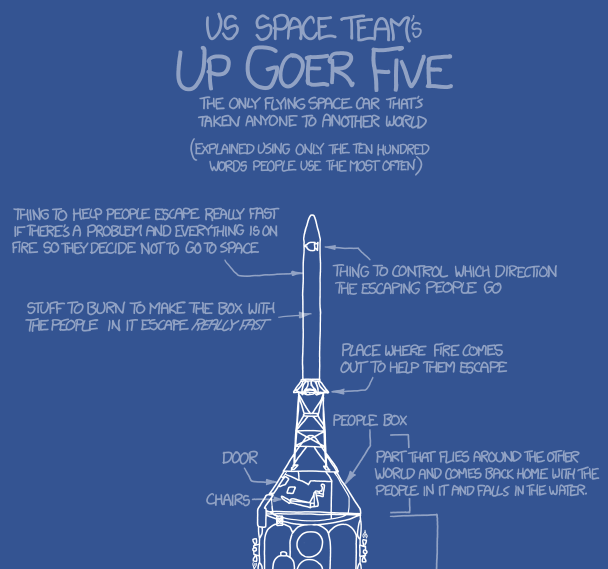
\includegraphics[width=\textwidth]{Slides/Design/Daten/up_goer_five_part.png}
	\end{figure}
	
	\column{0.4\textwidth}
	\begin{itemize}
		\item angemessene Leseschwierigkeit
		\begin{itemize}
			\item Satzlänge
			\item Wortlänge
			\item Vokabular
				%jargon, acronyme, worthäufigkeitslisten
		\end{itemize}
	\end{itemize}
\end{columns}
}
